% Style for a MSc paper at Warsaw School of Economics
% Michał Ramsza
% Friday, December 14, 2012

% --- document class and other global stuff ---------------------------
\documentclass[polish, twoside, 12pt, a4paper]{article}

%% --- packages --------------------------------------------------------
\usepackage{textcomp}
\usepackage{times}
\usepackage{amsmath}
\usepackage{amsfonts}
\usepackage{amssymb}
\usepackage{amsthm}
\usepackage[T1]{fontenc}
\usepackage[utf8]{inputenc}
\usepackage{graphicx}
\usepackage{xcolor}
\usepackage{enumitem}
\usepackage[polish]{babel}
\usepackage[centering, left=3.5cm, right=2.5cm, textheight=24cm]{geometry}
\usepackage{csvsimple}
\usepackage[T1]{fontenc}
% --- packages for citations ------------------------------------------
\usepackage[square,numbers]{natbib}
\AtBeginDocument{\renewcommand{\harvardand}{i}}

% --- package for automatic insertion of R code -----------------------
\usepackage{listings}
\lstset{language=R,%
   numbers=left,%
   tabsize=3,%
   numberstyle=\footnotesize,%
   basicstyle=\ttfamily \footnotesize \color{black},%
   escapeinside={(*@}{@*)}}

\begin{filecontents*}{grade.csv}
name,givenname,matriculation,gender,grade
Maier,Hans,12345,m,1.0
Huber,Anna,23456,f,2.3
Weisbaeck,Werner,34567,m,5.0
\end{filecontents*}


% --- support for links -----------------------------------------------
\usepackage{url}
\usepackage{hyperref}
\hypersetup{colorlinks=true,
            linkcolor=black,
            citecolor=darkgray,
            urlcolor=darkgray,
            pagecolor=darkgray}

% --- support for large tables and other stuff ------------------------
\usepackage{longtable}
% \usepackage{subfigure} % this package will not work with subcaption package
\usepackage{float}
\usepackage{caption}
\usepackage{subcaption}
\usepackage{wrapfig}
\usepackage{pdflscape} % relevant for wide tables (rotating pages)

% --- packages for game theory -----------------------------------------
\usepackage{sgame}

% --- support for no widows --------------------------------------------
\usepackage[defaultlines=4,all]{nowidow}

% --- quotation for polish language \enquote{}
\usepackage[autostyle]{csquotes}
\DeclareQuoteAlias{dutch}{polish}

% --- definitions for environments -------------------------------------
\theoremstyle{definition}
    \newtheorem{condition}{Założenie}
    \newtheorem{example}{Przykład}

\theoremstyle{plain}
    \newtheorem{definition}{Definicja}
    \newtheorem{proposition}{Stwierdzenie}
    \newtheorem{theorem}{Twierdzenie}
    \newtheorem{cor}{Wniosek}

\theoremstyle{remark}
    \newtheorem{remark}{Uwaga}

% --- other settings --------------------------------------------------
\linespread{1.5}
\frenchspacing
\sloppy
\allowdisplaybreaks[4]
\raggedbottom
\clubpenalty=10000
\widowpenalty=10000

% --- only if required ------------------------------------------------
\AtBeginDocument{\renewcommand*{\figurename}{Wykres}}
\AtBeginDocument{\renewcommand*{\tablename}{Tabela}}

% --- changing definition of footnote ---------------------------------
\makeatletter
\renewcommand\footnotesize{%
   \@setfontsize\footnotesize\@ixpt{10}%
   \abovedisplayskip 8\p@ \@plus2\p@ \@minus4\p@
   \abovedisplayshortskip \z@ \@plus\p@
   \belowdisplayshortskip 4\p@ \@plus2\p@ \@minus2\p@
   \def\@listi{\leftmargin\leftmargini
               \topsep 4\p@ \@plus2\p@ \@minus2\p@
               \parsep 2\p@ \@plus\p@ \@minus\p@
               \itemsep \parsep}%
   \belowdisplayskip \abovedisplayskip
}
\makeatother


% ---------------------------------------------------------------------
\begin{document}

% --- strona tytulowa -------------------------------------------------
\begin{titlepage}
\centering


\includegraphics[width=0.66\textwidth]{logo.JPG}

\vspace*{0.5cm}
Studium magisterskie\\
\begin{flushleft}
Kierunek: Metody Ilościowe w Ekonomii i Systemy Informacyjne\\
%Specjalność: <specjalność>
% Forma studiów: <forma studiów (stacjonarne, itd.)>
\end{flushleft}

\vspace*{.5cm}
\rule{0cm}{1cm}\hfill
\begin{minipage}{9cm}
Imie i nazwisko autora: Oskar Furmańczuk\\
Nr albumu: 81794
\end{minipage}

\vspace*{1cm}
\begin{minipage}{12cm}
\centering
\Large
\textbf{Determinanty przebiegu choroby COVID-19.}
\end{minipage}

\vspace*{2cm}
\rule{0cm}{1cm}\hfill
\begin{minipage}{9cm}
Praca licencjacka napisana\\
w Katedrze Matematyki i Ekonomii Matematycznej\\
pod kierunkiem naukowym\\
dr hab. Michała Ramszy
\end{minipage}

\vfill
Warszawa 2021
\end{titlepage}

\rule{1ex}{0ex}\clearpage

\graphicspath{ {./images/} }
% --- table of contents -----------------------------------------------
\cleardoublepage
\tableofcontents

% --- chapter ---------------------------------------------------------
\cleardoublepage
\section{Wprowdzenie}

- przegląd litertury dotyczącej koronawirusa - artykuły poświęcone badaniom wpływu czynników biologicznych na przebieg choroby \\
- związek pracy z ekonomią \\

% --- chapter ---------------------------------------------------------
\cleardoublepage
\section{Przegląd literatury}
\subsection{Rasa jako determinanta przebiegu choroby COVID-19 u pacjentów z chorobą współistniejącą}

Jednym z projektów prowadzonych na rzecz opisu przebiegu COVID-19 u pacjentów pochodzących z różnych grup rasowych jest „Racial disparities in patients with coronavirus disease 2019 infection and gynecologic malignancy”. Badanie to zostało przeprowadzone w Stanach Zjednoczonych na podstawie danych zebranych przez osiem systemów nowojorskich szpitali w okresie od 1 marca 2020 do 20 maja 202. Celem tego badania było sprawdzenie, czy istnieją rozbieżności na tle rasowym wśród pacjentek z rakiem ginekologicznym, u których stwierdzono obecność COVID-19.Wszystkie pacjentki biorące udział w badaniu miały ukończone 18 lat. Porównano charakterystykę wyjściową i kliniczną, zbadano różnice we wskaźnikach hospitalizacji i śmiertelności oraz wpływ rasy i innych czynników socjoekonomicznych i zdrowotnych na wyniki związane z COVID-19. 

Charakterystyka pacjentów obejmowała wiek, podawaną przez siebie rasę i pochodzenie etniczne, hrabstwo zamieszkania, status zatrudnienia, status pracownika zasadniczego, status ubezpieczenia, status mieszkaniowy, medyczne choroby współistniejące, ciężkość zakażenia COVID-19, typ raka, stadium rozpoznania, aktualny stan choroby nowotworowej i ostatnie leczenie przeciwnowotworowe.  Charakterystyka kliniczna COVID-19 obejmowała objawy COVID-19, parametry życiowe przy początkowym stadium choroby, powikłania szpitalne z powodu COVID-19 i konieczność stosowania dodatkowego tlenu, w tym inwazyjnej wentylacji mechanicznej. 

Rasę sklasyfikowano jako 2 grupy: czarnoskórzy versus nie-czarnoskórzy (biali plus pozostali). Zgrupowano pacjentów, którzy identyfikowali się jako Azjaci, Amerykańscy Indianie lub Rdzenni mieszkańcy Alaski, a także rdzenni Hawajczycy lub mieszkańcy Wysp Pacyfiku do innej grupy ze względu na niską liczbę w każdej kategorii. Biorąc pod uwagę wysoki odsetek białych w grupie innej niż czarna, rasy następnie podzielono na trzy grupy - czarnoskórzy, biali oraz pozostali. Łącznie 193 pacjentów - 67 czarnoskórych oraz 126 pozostałych.

Statystyki opisowe zostały obliczone dla cech demograficznych, socjoekonomicznych, zdrowotnych, związanych z nowotworem oraz związanych z COVID-19 u pacjentów rasy czarnej i innej niż czarna. Zmienne ciągłe zostały opisane jako mediany i przedziały międzykwartylowe (IQR) i zostały porównane między grupami za pomocą testu sumy rang Wilcoxona. Zmienne kategoryczne przedstawiono jako częstości i proporcje, a następnie zostały porównane między grupami za pomocą testu chi kwadrat. Wskaźniki hospitalizacji i śmiertelności obliczono wśród pacjentów rasy czarnej i innej niż czarna w populacji ogólnej lub w subpopulacji stratyfikowanej przez inne zmienne kategoryczne, a następnie porównano je za pomocą testu chi kwadrat.

Analiza wyników wykazała, iż nad 70\% pacjentów rasy czarnej w tym badaniu wymagało hospitalizacji z powodu zakażenia COVID-19, w porównaniu z zaledwie 46\% pacjentów rasy innej niż czarna. Oprócz rasy i wieku, zły stan sprawności i większa liczba chorób współistniejących wiązały się ze zwiększonym prawdopodobieństwem przyjęcia do szpitala. W szczególności, pacjenci rasy czarnej w wieku poniżej 65 lat prawie 5 razy częściej wymagali hospitalizacji z powodu COVID-19 w porównaniu z pacjentami rasy czarnej w tym samym wieku. Rasa czarna nie była związana ze zwiększoną śmiertelnością z powodu COVID-19 przed lub po skorygowaniu o cechy kliniczne i socjoekonomiczne. Badanie wykazało, że pacjenci rasy czarnej są od 2 do 3 razy bardziej narażeni na konieczność hospitalizacji niż pacjenci rasy białej po skorygowaniu czynników zakłócających, w tym wieku, płci, chorób współistniejących i dochodów, a prawdopodobieństwo ich śmierci z powodu zakażenia COVID-19 jest ponad 5 razy większe.

%---obrazek---------

\begin{figure}[h]
\centering
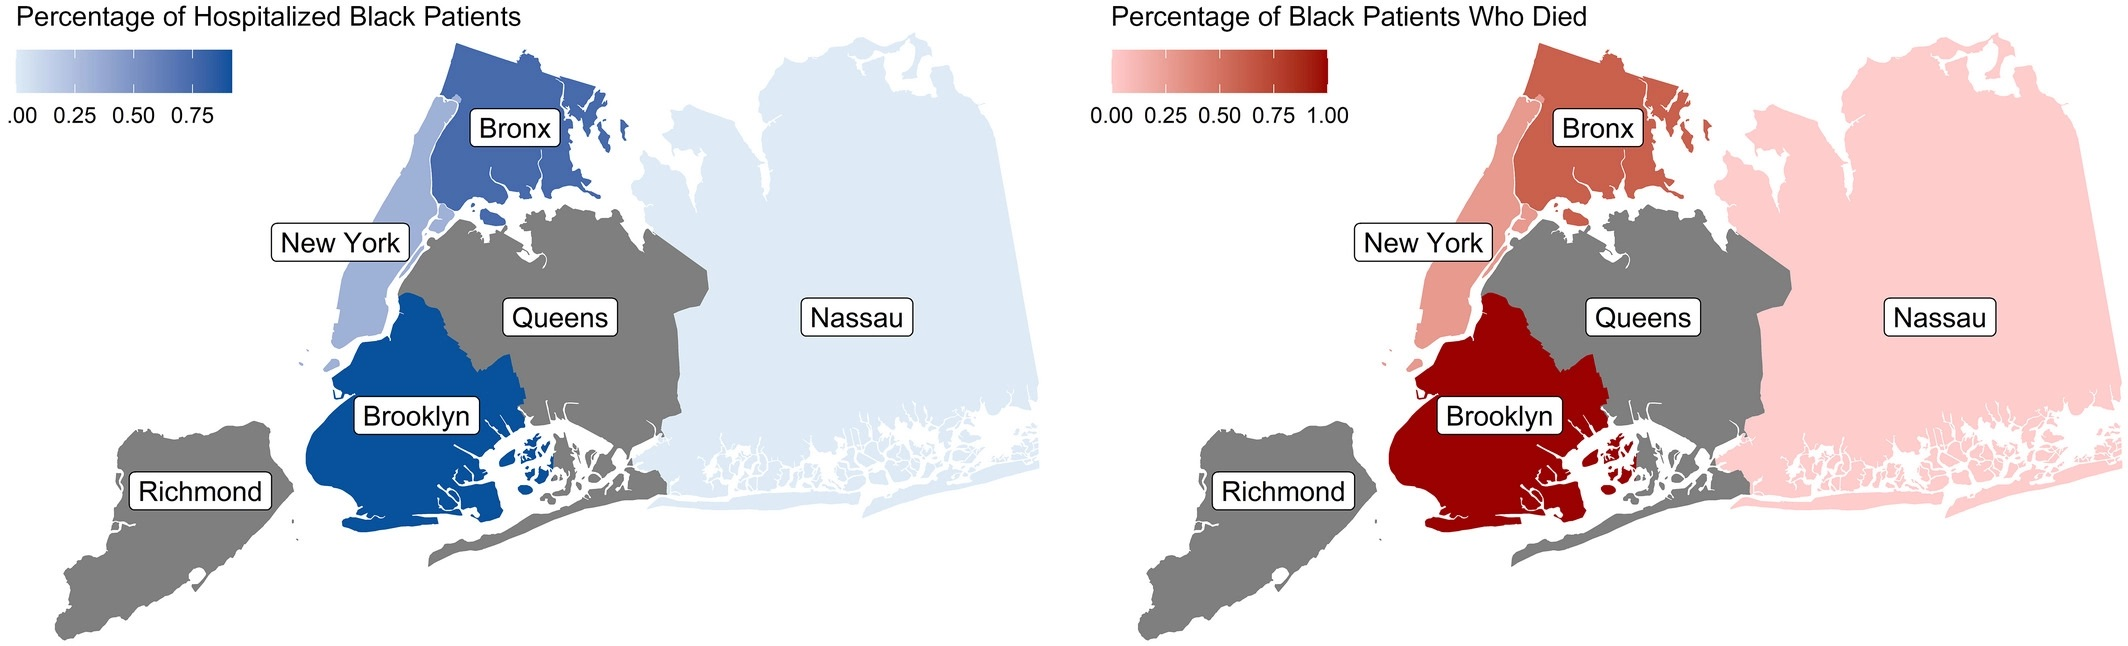
\includegraphics[width=15cm]{NY-racial-disparities.jpg}
\caption{Odsetki hospitalizacji (po lewej) i dane dotyczące śmiertelności (po prawej) zilustrowane dla pacjentów rasy czarnej w badanych dzielnicach Nowego Yorku (USA)}
\end{figure}

Autorzy badania wskazują za przyczynę gorszych rokowań czarnoskórych czynniki takie jak ograniczony dostęp do świadczeń opieki zdrowotnej, strukturalne i społeczne uwarunkowania opieki medycznej, rasizm i dyskryminację. Ponadto, Afroamerykanie są bardziej narażeni na współistniejące choroby medyczne, o których wiadomo, że są czynnikami ryzyka ciężkiego zakażenia COVID-19, w tym nadciśnienie tętnicze, cukrzycę, choroby nerek i układu oddechowego. W tej grupie badawczej większy odsetek czarnych pacjentów w wieku poniżej 65 lat miał więcej niż 3 współistniejące choroby i charakteryzował się większą częstością występowania nadciśnienia tętniczego, otyłości i cukrzycy w porównaniu z pacjentami rasy innej niż czarna w tej grupie wiekowej. Czarnoskórzy pacjenci mieli również częściej zamieszkiwali obszary poniżej granicy ubóstwa. \cite{borghesi2020}

\subsection{Wpływ wieku oraz płci na przebieg COVID-19}

Jednym z badań które zgłębia przebieg infekcji COVID-19 u pacjentów różnej płci z podziałem na grupy wiekowe jest "Radiographic severity index in COVID-19 pneumonia: relationship to age and sex in 783 Italian patients". Badnie zostało przeprowadzone na grupie 783 (532 mężczyzn i 251 kobiet) włoskich pacjentów z laboratoryjnie stwierdzonym COVID-19. Osoby poniżej 20 roku życia zostali wykluczeni z badania. Pozostali pacjenci zostali podzieleni na 7 grup wiekowych: 20-29 lat (grupa A), 30-39 lat (grupa B), 40-49 lat (grupa C), 50-59 lat (grupa D), 60-69 lat (grupa E), 70-79 lat (grupa F) oraz powyżej 80 lat (grupa G). Do interpretacji stanu pacjenta posłużono się osiemnasto-poziomowym wskaźnikiem oceny sprawności płuc uzyskiwanym przez analizę prześwietleń klatki piersiowej (dalej: CXR).

Mediana wieku wynosiła 65 lat (zakres międzykwartylowy, 55-74 lata). Spośród włączonych pacjentów, 10 (1,3\%) było z grupy A, 29 (3,7\%) z grupy B, 80 (10,2\%) z grupy C, 168 (21,5\%) z grupy D, 196 (25\%) z grupy E, 210 (26,8\%) z grupy F i 90 (11,5\%) z grupy G. Dla każdej grupy, test Manna-Whitneya U został użyty do porównania wyników CXR mężczyzn i kobiet. Korelacja rang Spearmana została zastosowana do oceny zależności pomiędzy wynikiem CXR a wiekiem. Test Kruskala-Wallisa zastosowano również w celu określenia, czy istnieją istotne różnice w punktacji CXR pomiędzy grupami wiekowymi. Wartości p $\leq$ 0,05 uznano za istotne statystycznie.

Wynik CXR był istotnie wyższy u mężczyzn niż u kobiet tylko w grupach D, E i F (p < 0,020). Stwierdzono istotną korelację między wynikiem CXR a wiekiem zarówno u mężczyzn, jak i u kobiet (rho = 0,205, p < 0,0001 dla mężczyzn; rho = 0,310, p < 0,0001). U mężczyzn wynik CXR w grupach D, E, F i G był znamiennie wyższy niż w grupach A, B i C (ryc. 3). U kobiet wynik CXR w grupach E, F i G był znamiennie wyższy niż w grupach A i B (ryc. 3). Wynik CXR w grupie G był również znamiennie wyższy niż w grupach C, D i E. Wynik CXR w grupie F był znamiennie wyższy niż w grupie C.

\begin{figure}[h]
\centering
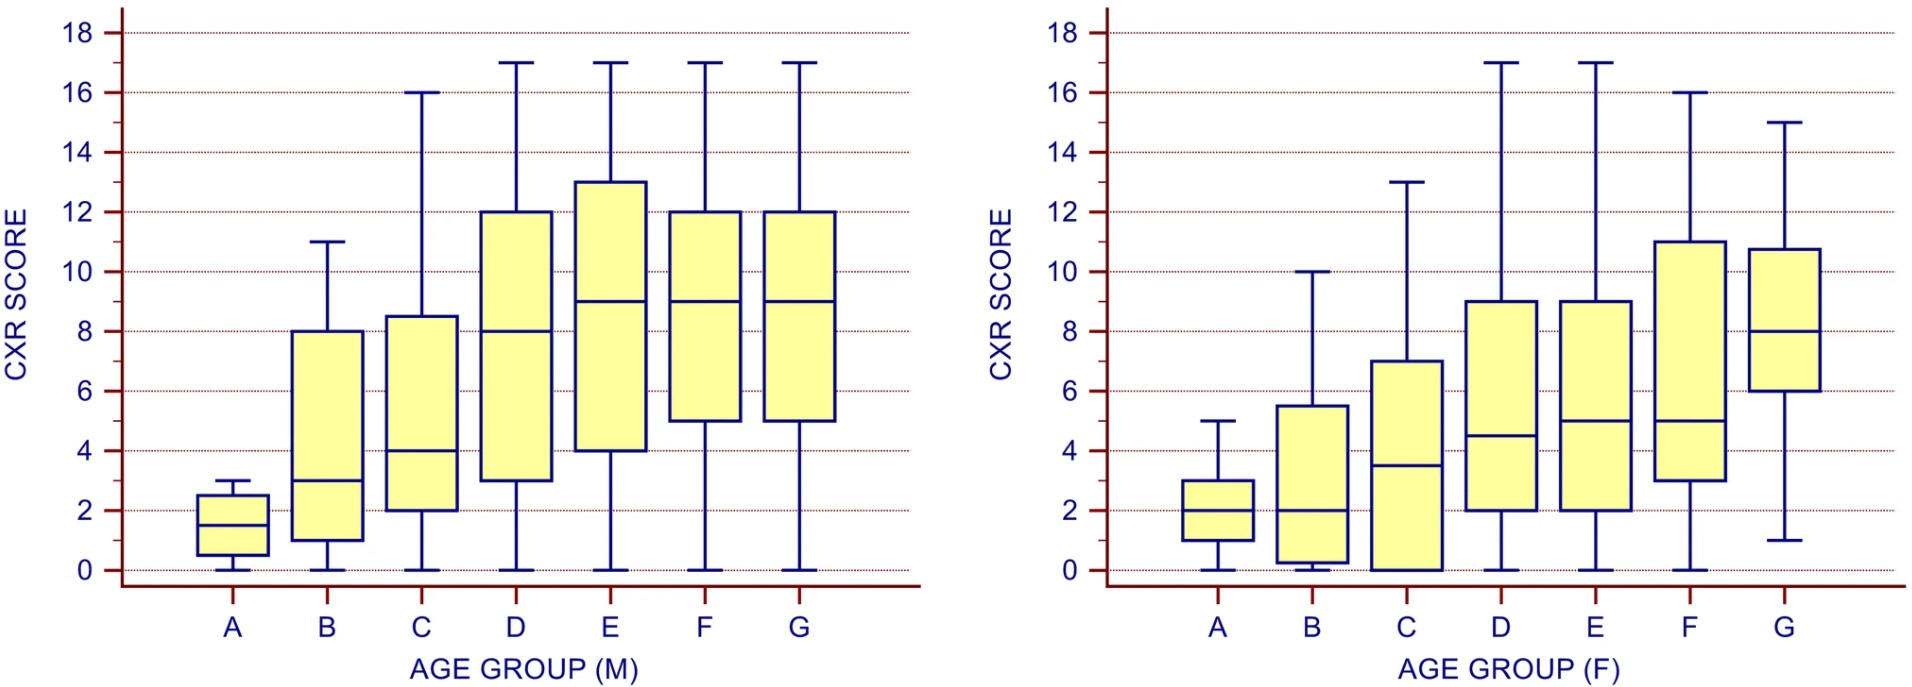
\includegraphics[width=15cm]{age-sex.jpg}
\caption{Rozkład wyników badania RTG klatki piersiowej (CXR) w zależności od grupy wiekowej u mężczyzn (M) i kobiet (F)}
\end{figure}

Podsumowując, autorzy badania wskazują na istotny wpływ wieku na śmiertelność przy infekcji COVID-19. Stwierdzono, że mężczyźni w wieku 50 lat lub starsi i kobiety w wieku 80 lat lub starsze wykazywali najwyższe ryzyko rozwoju ciężkiej choroby płuc. \cite{wang2020}

\subsection{Zmienne meteorologiczne jako determinanty częstotliwości zachorowań na COVID-19}

Opublikowany w wrześniu 2020 artykuł „Effect of meteorological factors on COVID-19 cases in Bangladesh” koncertuje się na opisie wpływu warunków pogodowych na możliwość zarażenia się koronawirusem. Badanie na temat którego powstał wspomniany artykuł przeprowadzono na terytorium Bangladeszu. Kraj znajduję się w strefie klimatu zwrotnikowego, a na jego terytorium występują 3 główne pory roku: pre-monsun,monsun, post-mosum. Ze względu na złożone warunki klimatyczne i dużą gęstość zaludnienia obszar ten jest uznawany za wysoce wrażliwy na zmiany klimatu.

Do przeprowadzenia badania zebrano dane z 43 stacji meteorologicznych z których wyodrębniono informacje na temat kilkunastu parametrów atmosferycznych (maksymalna temperatura dobowa (MaxT), minimalna temperatura dobowa (MinT), siła wiatru (WS), wilgotność relatywna (RH), wilgotność absolutna (AH) itp.) dla odpowiadającym im regionów. Na podstawie danych o przypadkach zachorowani na COVID-19 z odpowiadających im obszarów ustalono wskaźnik relatywnego ryzyka (RR), który oceniał prawdopodobieństwo zarażenia się SARS-CoV-2 w określonym dniu. Ze względu na od 2 do 14 dniowy okres inkubacji wirusa przyjęto maksymalnie 14 dniowe opóźnienie między obserwacjami meteorologicznymi, a poszczególnymi przypadkami zgłoszonych zachorowań.

Koherencja transformaty falkowej (WTC) i częściowa koherencja falkowa (PWC) zostały wykorzystane w tym badaniu do uzyskania wyrazów rozdzielczości czasowej i częstotliwościowej zmiennych klimatycznych i przypadków COVID-19 w Bangladeszu. WTC kwantyfikuje wielkość kowariancji między dwoma szeregami czasowymi, która waha się od 0 do 1 (0 $\leq$ R2 $\leq$ 1). 0 odnosi się do całkowitego braku spójności, podczas gdy 1 odnosi się do doskonałej spójności. Zakres ten definiuje się jako kwadrat widma krzyżowego znormalizowanego przez wygładzone indywidualne widmo mocy. 

RH wykazało silny pozytywny znaczący związek z przypadkami COVID-19 w Singapurze. Oznacza to, że maksymalne RH (71,4 $\pm$ 4\%) w maju sprzyjało rozprzestrzenianiu się COVID-19. WS wykazał znaczący związek z potwierdzonymi przypadkami COVID-19 w Bangladeszu. Natomiast AP wykazywał stosunkowo silną odwrotną zależność z pozytywnymi przypadkami zakażenia COVID-19 w Bangladeszu w początkowej fazie epidemii SARS-CoV-2. Ogólnie rzecz biorąc, wysokie wartości MinT, RH i AH wraz z niskimi WS w maju nasiliły rozprzestrzenianie się SARS-CoV-2.

Przedstawiono zależność opóźnionej odpowiedzi RR na wzrost o 1 jednostkę wszystkich wskaźników meteorologicznych w różnych dniach opóźnienia (do 14 dni). Największe RR dla MaxT wyniosło 1,00 (95\% CI 0,99-1,01) w opóźnieniu 6-dniowym, a najmniejsze 0,92 (95\% CI 0,88-0,95) bez opóźnienia. Największe RR dla MinT wyniosło 1,04 (95\% CI 1,01-1,06) w opóźnieniu 11-dniowym, a najmniejsze 1,01 (95\% CI 0,99-1,02) w opóźnieniu 2-dniowym. 

\begin{figure}[h]
\centering
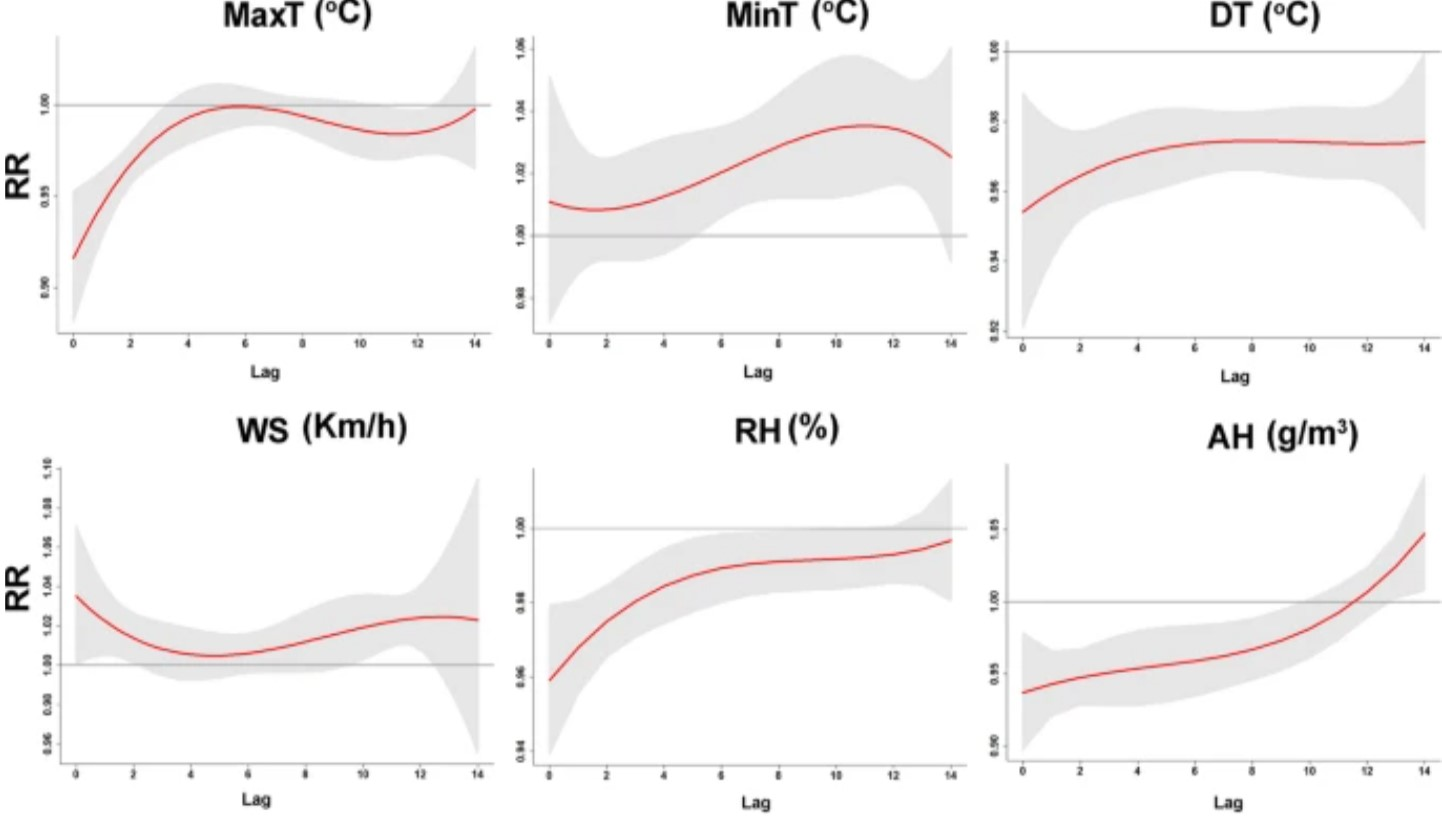
\includegraphics[width=15cm]{clmate-factors.jpg}
\caption{Pojedyncze efekty MaxT, MinT, DT, WS, RH i AH. Laboratorium Y oznacza wartość ryzyka względnego (RR)}
\end{figure}

Podsumowując, zaobserwowano znaczący wpływ pomiędzy COVID-19 a zmiennymi meteorologicznymi. Temperatura, może odgrywać istotną rolę w procesach życiowych człowieka oraz w zakresie ograniczania i kontroli epidemii. Ponadto, oddnotowano wpływ siły wiatru na propagowanie epidemii. Wiatr może wpływać na czas zawieszenia koronawirusa i jego rozprzestrzenianie się. Badanie wykazało, że wskaźnik RR wyraźnie wzrósł, w czasie gdy WS podwyższył się o ponad 21 km/h. Stężenie koronawirusa może być rozcieńczone przez podwyższony WS, co może stanowić prawdopodobne wyjaśnienie tego wyniku. Można wnioskować, iż temperatura i prędkość wiatru wykazują silny związek z wybuchem i przebiegiem epidemii COVID-19 w Bangladeszu. \cite{hasanuzzaman2020}



% --- chapter ---------------------------------------------------------
\clearpage
\section{Opis zbioru danych}

- liczebność oraz źródło zbioru danych \\
- opisy zmiennych \\
- rozkład zmiennych \\
- charakterystyki zmiennych (np. średnie, odchylenia std ) \\
- charakterystyka brakujących danych \\
- problemy wynikające z brakujących danych


Do przeprowadzenia badania zostały użyte 3 zbiory danych: 
\begin{itemize}
  \item dane na temat poszczególnych przypadków zachorowań na COVID-19 w USA - pochodzą z zasobów Centers for Disease Control and Prevention
  \item wskaźniki atmosferyczne dla poszczególnych części USA - pochodzą z zasobów National Centers for Environmental Information
  \item dane demograficzne  dla poszczególnych części USA - pochodzą z portalu ArcGis
\end{itemize}



\subsection{Zbiór danych dotyczący poszczególnych przypadków zachorowań na COVID-19}


Zbiór danych pochodzi z zastrzeżonych zasobów Centers for Disease Control and Prevention (CDC). Zbiór ten został udostępniony po bezpośredniej prośbie skierowanej do jego właścicieli i za ich pozwoleniem został wykorzystany w tej pracy. Zebrane są w nim podstawowe dane medyczne osób ze stwierdzonym COVID-19 zarejestrowanych przez amerykańską służbę zdrowia z okresu od pierwszego potwierdzonego przypadku zachorowania (styczeń 2020) do końca lutego 2021 roku - łącznie 20,5 mln obserwacji. Zmienne, które zostały użyte w tej pracy zostały scharakteryzowane w tabeli \ref{table:zmienneCDC} .

\begin{table}[H]
  \centering
\resizebox{15cm}{!}{
\centering
\csvautotabular[respect underscore=true]{a.csv}
}
\caption{Zmienne ze zbioru CDC użyte w dalszej części pracy.}
\label{table:zmienneCDC}
\end{table}

W zbiorze danych występują 3 typy brakujących danych. Najczęściej występującym jest \emph{Unknown} i jak autor zbioru danych opisuje kodowany był w przypadku udzielenia dokładnie takiej odpowiedzi do pytania szpitalnej ankiety. Kolejnym typem jest  \emph{Missing} i występuję w przypadkach nie udzielenia jakiejkolwiek odpowiedzi. Najrzadziej występującym typem wskazującym brak danych jest \emph{NaN} i zakodowany został w miejscach logicznej nieścisłości danych oraz w przypadkach błędów na poziomie zapisu danych w centralnej bazie.

Pomimo bardzo dużej ilości obserwacji wadą zbioru okazał się niski udział w pełni opisanych przypadków (większość zmiennych zawiera mniej niż 25\% uzupełnionych danych). Obliczone częstości występowania oraz korelacje brakujących danych pomiędzy zmiennymi z uwzględnieniem oraz bez uwzględnienia typów braków danych nie wskazała przyczyny dużego natężenia braku danych. Uznano również, że lokalizacja brakujących danych jest niedeterministyczna. Ze względu na jakościową naturę zmiennych oraz wysoki udział brakujących danych nie możliwe było przeprowadzenie imputacji brakujących danych. Znikoma wartość informacja niesiona przez brak danych przyczyniłaby się do zaburzenia interpretacji wyników dalszej części pracy dlatego podjęto decyzję o odrzuceniu wszystkich niepełnych obserwacji. Dalsza część pracy odnosi się do wyselekcjonowanych tym sposobem 171 147 pełnych obserwacji. 

W zbiorze udostępnionym przez CDC pacjenci zostali podzieleni na 8 grup wiekowych o rozpiętości 10 lat, a dla najstarszych stworzono grupę 80+. Zmienna \emph{race\_ethnicity\_combined} przyjmuje wartości: \emph{American Indian/Alaska Native, Non-Hispanic} dla natywnych mieszkańców Ameryki Północnej, \emph{Asian, Non-Hispanic} dla rasy żółtej, \emph{Black, Non-Hispanic} dla rasy czarnej, \emph{Hispanic/Latino} dla mniejszości latynoskiej, \emph{Native Hawaiian/Other Pacific Islander, Non-Hispanic} dla natywnych mieszkańców wysp Pacyfiku, \emph{White, Non-Hispanic} dla rasy białej oraz \emph{Multiple/Other, Non-Hispanic} dla pozostałych. Wartości zmiennej \emph{sex} zostały przekodowane na 1 dla mężczyzn oraz 0 dla kobiet. Wartości dla pozostałych zmiennych dwumianowych zostały przekodowane na 1 dla wartości \emph{Yes} oraz na 0 dla \emph{No}.

Najliczniejszą grupą w zbiorze okazali się być przedstawiciele rasy białej i składają się na 73.8\% wszystkich obserwacji. Natywni mieszkańcy wysp Pacyfiku (0,38\%) oraz natywni mieszkańcy Ameryki Północnej (0,11\%) stanowią najmniej liczne grupy etniczne w opisywanym zbiorze danych. Udział procentowy kobiet jest porównywalny do udziału mężczyzn i wynosi odpowiednio 44,2\% dla mężczyzn oraz 55,8\% dla kobiet (Wykres: \ref{figure:sex-race-count})

\begin{figure}[H]
\centering
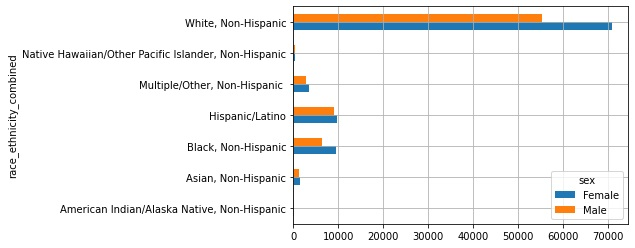
\includegraphics[width=15cm]{race_sex_count_plot.jpg}
\caption{Liczebność poszczególnych grup etniczno-rasowych z podziałem na płeć}
\label{figure:sex-race-count}
\end{figure}

Najczęstszymi symptomami COVID-19 był kaszel (60,9\%), ból głowy (59,0\%) oraz bóle mięśniowe (53.1\%). Najrzadziej pacjenci informowali o dolegliwościach związanych z bólem brzucha (11,5\%) oraz nudnościami (21,5\%) W opisanym zbiorze wskaźnik hospitalizacji wyniósł 6,72\%, a wskaźnik śmiertelności 1,28\%.

\begin{figure}[H]
\centering
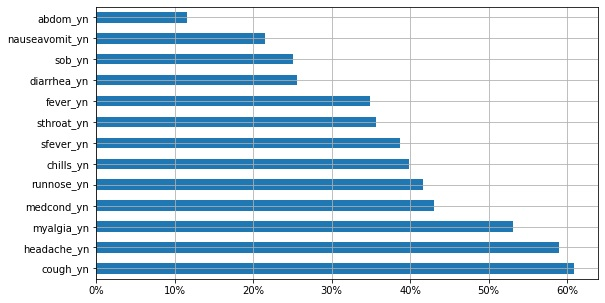
\includegraphics[width=15cm]{symptoms-freq.jpg}
\caption{Częstość występowania poszczególnych objawów COVID-19}
\end{figure}



\subsection{Zbiory danych zawierający wskaźniki atmosferyczne dla poszczególnych części USA}

Kolejne zbiory danych jakie użyto w tej pracy pochodzą z upublicznionych zasobów National Centers For Environmental Information. Zawierają one dane na temat najważniejszych parametrów metrologicznych obserwowanych przez największe miasta USA. Udostępnione dane zawierają średnie wartości zagregowane na poziomie miesięcznym i rocznym. Korzystając z tego źródła do tej pracy użyto trzech poniższych tabel:
\begin{itemize}
  \item \emph{Normal Daily Maximum Temperature, °F} - średnie dobowe temperatury obliczone na podstawie obserwacji zebranych w latach 1971-2000 wyrażone w stopniach Fahrenheita.
  \item \emph{Wind - Average Speed (MPH)} - średnie prędkości wiatru obliczone bez uwzględnienia jego kierunku wyrażone w milach na godzinę.
  \item \emph{Average Relative Humidity (Percent) - Morning (M) and Afternoon (A)} - średnie wilgotności powietrza rano i wieczorem obliczone wyrażone w procentach.
\end{itemize}

Ze względu na fakt, iż dla niektórych hrabstw nie odnotowano żadnych obserwacji postanowiono zgrupować dane na poziomie stanów i wyliczyć dla nich średnie wartości. W zestawieniu rocznym najgorętszym stanem okazała się Floryda osiągając średnią temperaturę 72,1 \textdegree F (22,3 \textdegree C), najchłodniejszym zaś Alaska ze średnią temperaturą 32,8 \textdegree F (0,4 \textdegree C). Największa średnia roczna prędkość wiatru przypada na stan Kansas (11,2 mph) i Massachusetts (10,9 mph), najmniejsza zaś w stanie West Virginia (5,6 mph). 

\begin{figure}[H]
\centering
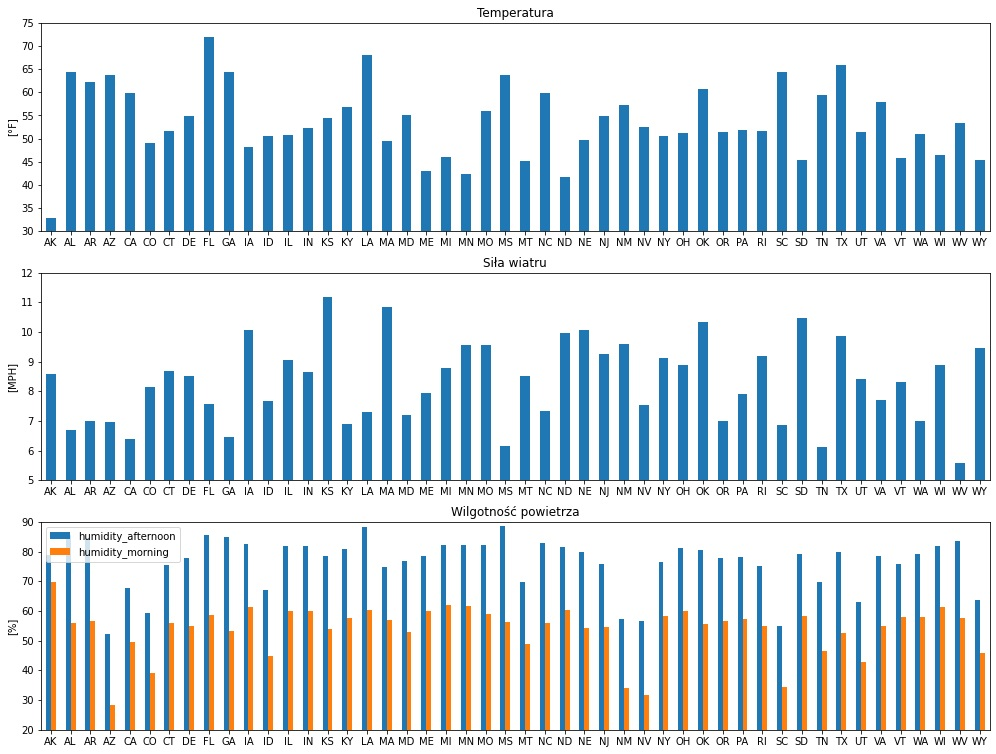
\includegraphics[width=15cm]{atm-all.jpg}
\caption{Wybrane wskaźniki atmosferyczne zagregowane na poziomie rocznym zgrupowane dla poszczególnych stanów. }
\end{figure}


\subsection{Zbiór danych zawierający dane demograficzne}

Ostatnim zbiorem jaki został wykorzystany w tej pracy jest zbiór \emph{USA Counties} pochodzący z ArcGIS Hub. Autorem zbioru jest ArcGIS Data and Maps (poprzednio Esri Data \& Maps), czyli sam zespół portalu ArcGIS. Oprócz danych demograficznych w zbiorze znaleźć można dane geograficzne oraz wskaźniki związane z rolnictwem. Dane demograficzne datowane są na 2010 rok i pochodzą z amerykańskiego spisu powszechnego. Wszystkie zmienne zostały określone na poziomie hrabstw.

Ze względu na tematykę pracy postanowiono wykorzystać z opisanego zbioru tylko jedną zmienną, czyli \emph{POP\_SQMI} - zagęszczenie ludności na mile kwadratową. Analiza zbioru wykazała, że najmniej rzadziej zaludnione hrabstwa w USA to Lake and Peninsula, North Slope, Denali, Yakutat oraz Loving z gęstością zaludnienia na poziomie 0,1 osoby na mile kwadratowej. Wszystkie wymienione hrabstwa oprócz Loving (stan Texas) zlokalizowane są na obszarze Alaski. Najgęściej zaludnione hrabstwa to New York (73032,2 osoby na mile kwadratową), Kings (38512,3 osoby na mile kwadratową) oraz Bronx (34919,1 osoby na mile kwadratową) - wszystkie zlokalizowane w stanie New York. Gęstość zaludnienia Stanów Zjednoczonych, obliczona przez zsumowanie populacji wszystkich hrabstw i podzielenie przez sumę ich powierzchni, wynosi 91,1 osoby na mile kwadratową.

\begin{figure}[H]
\centering
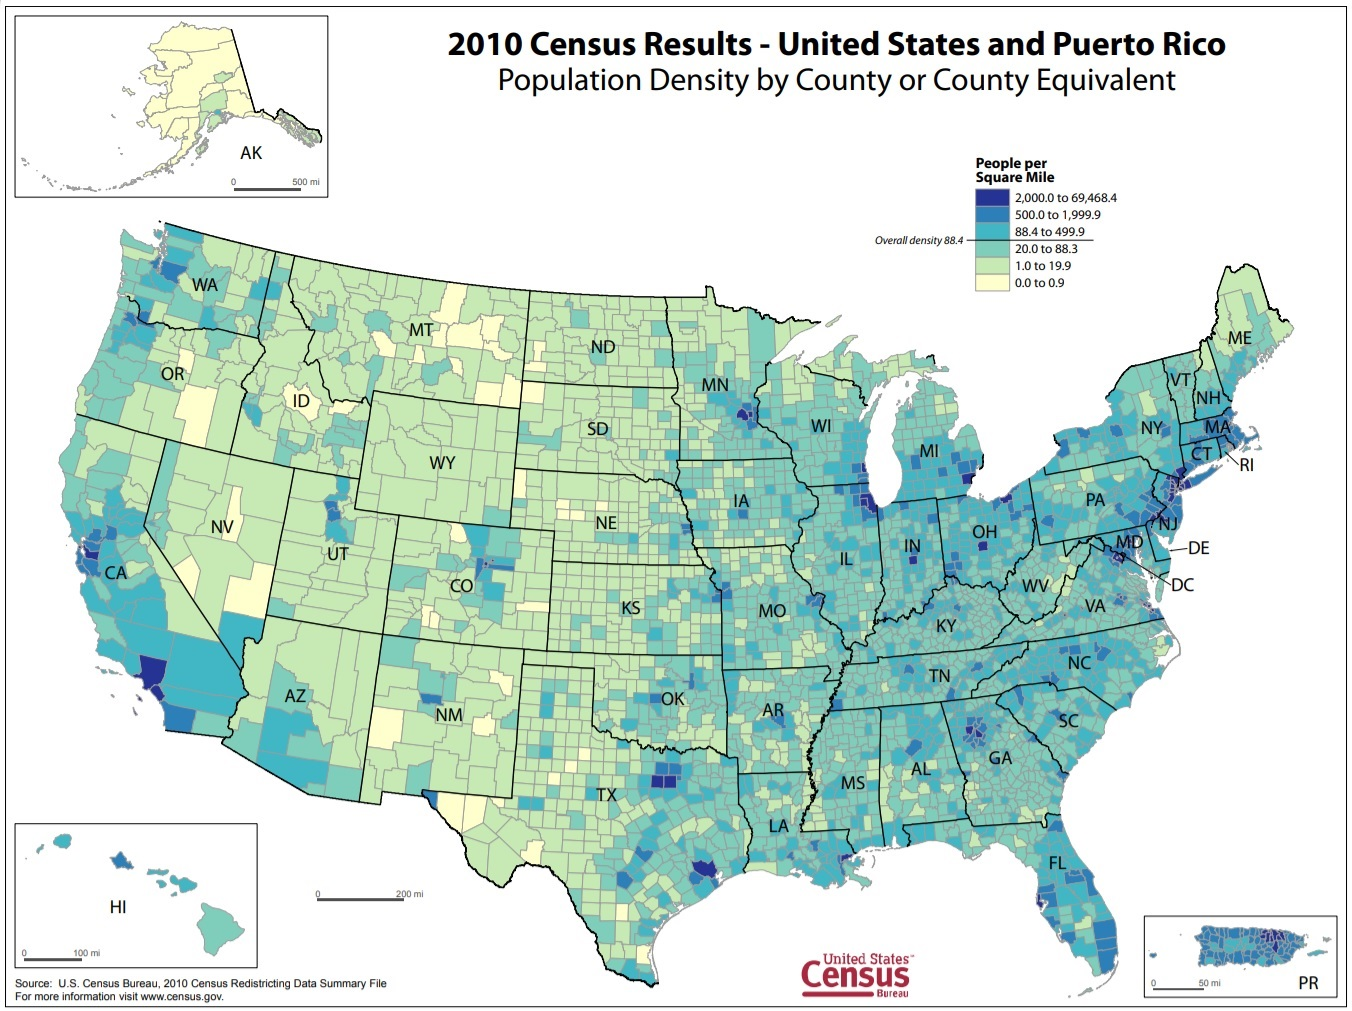
\includegraphics[width=15cm]{us-desity.jpg}
\caption{Zagęszczenie ludności zwizualizowane na mapie Stanów Zjednoczonych. }
\end{figure}

\subsection{Docelowy zbiór danych}

Po uzyskaniu zbiorów z zewnętrznych zasobów oraz wstępnego oczyszczenia danych postanowiono stworzyć zbiór danych, który posłuży do budowy modelu XGBoost. Podstawą do budowy tego zasobu był zbiór danych związany z poszczególnymi obserwacjami zachorowań COVID-19 do którego dowiązano w określony sposób pozostałe zbiory zbiory.

Pierwszym krokiem było dowiązanie wskaźników atmosferycznych do zbioru danych związanego z obserwacjami COVID-19 . Dokonano tego przez zmapowanie miesiąca zachorowania i zamieszkanego stanu ze wskazaną zmienną meteorologiczną przypisaną dla tego stanu w tym terminie. W ten sposób otrzymano następujące zmienne:
\begin{itemize}
  \item \emph{avg\_temp} - średnia dobowa temperatura wyrażona w stopniach Fahrenheita.
  \item \emph{avg\_wind} - średnia prędkość wiatru wyrażona w milach na godzinę.
  \item \emph{avg\_humidity\_M} - średnia wilgotność powietrza rano wyrażona w procentach.
  \item \emph{avg\_humidity\_A} - średnia wilgotność powietrza wieczorem wyrażona w procentach.
\end{itemize}

Kolejnym etapem było dowiązanie powstałego w poprzednim kroku zbioru ze zbiorem danych uzyskanym z portalu ArcGIS. Osiągnięto to przez zmapowanie nazwy zamieszkanego hrabstwa osoby ze stwierdzonym COVID-19 z gęstością zaludnienia w tym obszarze. W ten sposób uzyskano zmienną \emph{pop\_density}, która określa gęstość zaludnienia wyrażoną w liczbie osób na mile kwadratową.

Ostatnim krokiem było odrzucenie niepożądanych zmiennych z powstałego zbioru danych. Ten etap był konieczny gdyż niektóre zmienne nie miały bezpośredniego związku z wyjaśnieniem przedmiotu tej pracy. Odrzuconymi zmiennymi były:  \emph{county\_fips\_code},  \emph{res\_county}, \emph{res\_state}, \emph{cdc\_case\_earliest\_dt}, \emph{date\_month} oraz \emph{current\_status}.

% --- chapter ---------------------------------------------------------
\clearpage
\section{Metody}

- opis kolejności obliczeń/transformacji/budowy modelu \\
- opis użytego modelu (docelowo: xgboost) oraz jego zasadność względem niezbalansowanej próby\\
- opis metod walidacji oraz jakości modelu (F1-score, accuracy) \\
- opis sposobu interpretacji wpływu zmiennych objaśniających na zmienną objaśnianą (docelowo: SHAP)

% --- chapter ---------------------------------------------------------
\clearpage
\section{Wyniki i dyskusja}

- przedstawienie wzkaźników jakości modelu \\
- przstawienie wyników SHAP oraz ich interpretacja \\
- porównanie wniosków uzyskanych z opracowanego modelu z wnioskami z przywołanej literatury naukowej \\ 

% --- chapter ---------------------------------------------------------
\clearpage
\section{Zakończenie}


- podsumowanie pracy \\


% --- chapter -------
--------------------------------------------------
\clearpage
\section{Literatura}



% --- appendices ------------------------------------------------------
\appendix

% ---------------------------------------------------------------------
\clearpage
\section{Dodatek: Ważne rzeczy do dodania}




% --- bibliography ----------------------------------------------------
\clearpage
\bibliographystyle{agsm}
\bibliography{refs}

% --- abstract --------------------------------------------------------
\clearpage
\addcontentsline{toc}{section}{Lista tablic}
\listoftables

% --- abstract --------------------------------------------------------
\clearpage
\addcontentsline{toc}{section}{Lista rysunków}
\listoffigures



% --- abstract --------------------------------------------------------
\clearpage
\addcontentsline{toc}{section}{Streszczenie}
\section*{Streszczenie}

Tutaj zamieszczają Państwo streszczenie pracy. Streszczenie powinno być długości około pół strony.


\end{document}

%%% Local Variables:
%%% mode: latex
%%% TeX-master: t
%%% End:
